\documentclass[11pt,a4paper]{report}
\title{ZUArm}
\author{Osama Yousry \and Aly Mahmoud Samy \and Ashraf Saeed Teleb \and Merihan Sadek \and Sara AbdelHamid \and Shaimaa Askar \and Youssef Alaa-ElDin \and Mohammed Hessein \and Mohammed Gameel} 

%\usepackage{fancyhdr}
\usepackage{graphicx}
\usepackage{hyperref}
\usepackage{listings}
\usepackage{color}
%\usepackage[demo]{graphicx}
\usepackage{caption}
\usepackage{subcaption}
\usepackage{amsmath}
\usepackage{amssymb}
\definecolor{dkgreen}{rgb}{0,0.6,0}
\definecolor{gray}{rgb}{0.5,0.5,0.5}
\definecolor{mauve}{rgb}{0.58,0,0.82}


\renewcommand\thesection{\arabic{section}}


\lstset{frame=none,
  language=C++,
  aboveskip=3mm,
  belowskip=3mm,
  showstringspaces=false,
  columns=flexible,
  basicstyle={\small\ttfamily},
  numbers=none,
  numberstyle=\tiny\color{gray},
  keywordstyle=\color{blue},
  commentstyle=\color{dkgreen},
  stringstyle=\color{mauve},
  breaklines=true,
  breakatwhitespace=true,
  tabsize=3
}


\begin{document}
%\maketitle
\begin{titlepage}
	\centering
		
\includegraphics[width=0.15\textwidth]{zuLogo.jpg}
\par\vspace{1cm}
	{\scshape\LARGE Zagazig University \par}
	\vspace{1cm}
	{\scshape\Large Robotics project\par}
	\vspace{1.5cm}
	{\huge\bfseries ZUArm\par}
	\vspace{2cm}
	{\itshape Osama Yousry\\
	Aly Mahmoud Samy\\
	Ashraf Saeed Teleb\\
	Merihan Sadek\\
	Mohammed Gameel\\
	Mohammed Hesssein\\
	Sara AbdelHamid\\
	Shaimaa Askar\\
	Youssef Alaa-Eldin\\}
	\vfill
	supervised by\par
	Dr.~Mohamed \textsc{Nour}

	\vfill

% Bottom of the page
	{\large \today\par}
\end{titlepage}
%\listoffigures
%\listoftables
%\tableofcontents
\section{Introduction}
ZUArm is a robotics mini-project built on an older robotic arm project, implemented to demonstrate basic understanding of the robotics curriculum.
\section{Description}
\begin{figure}[h]
\centering
{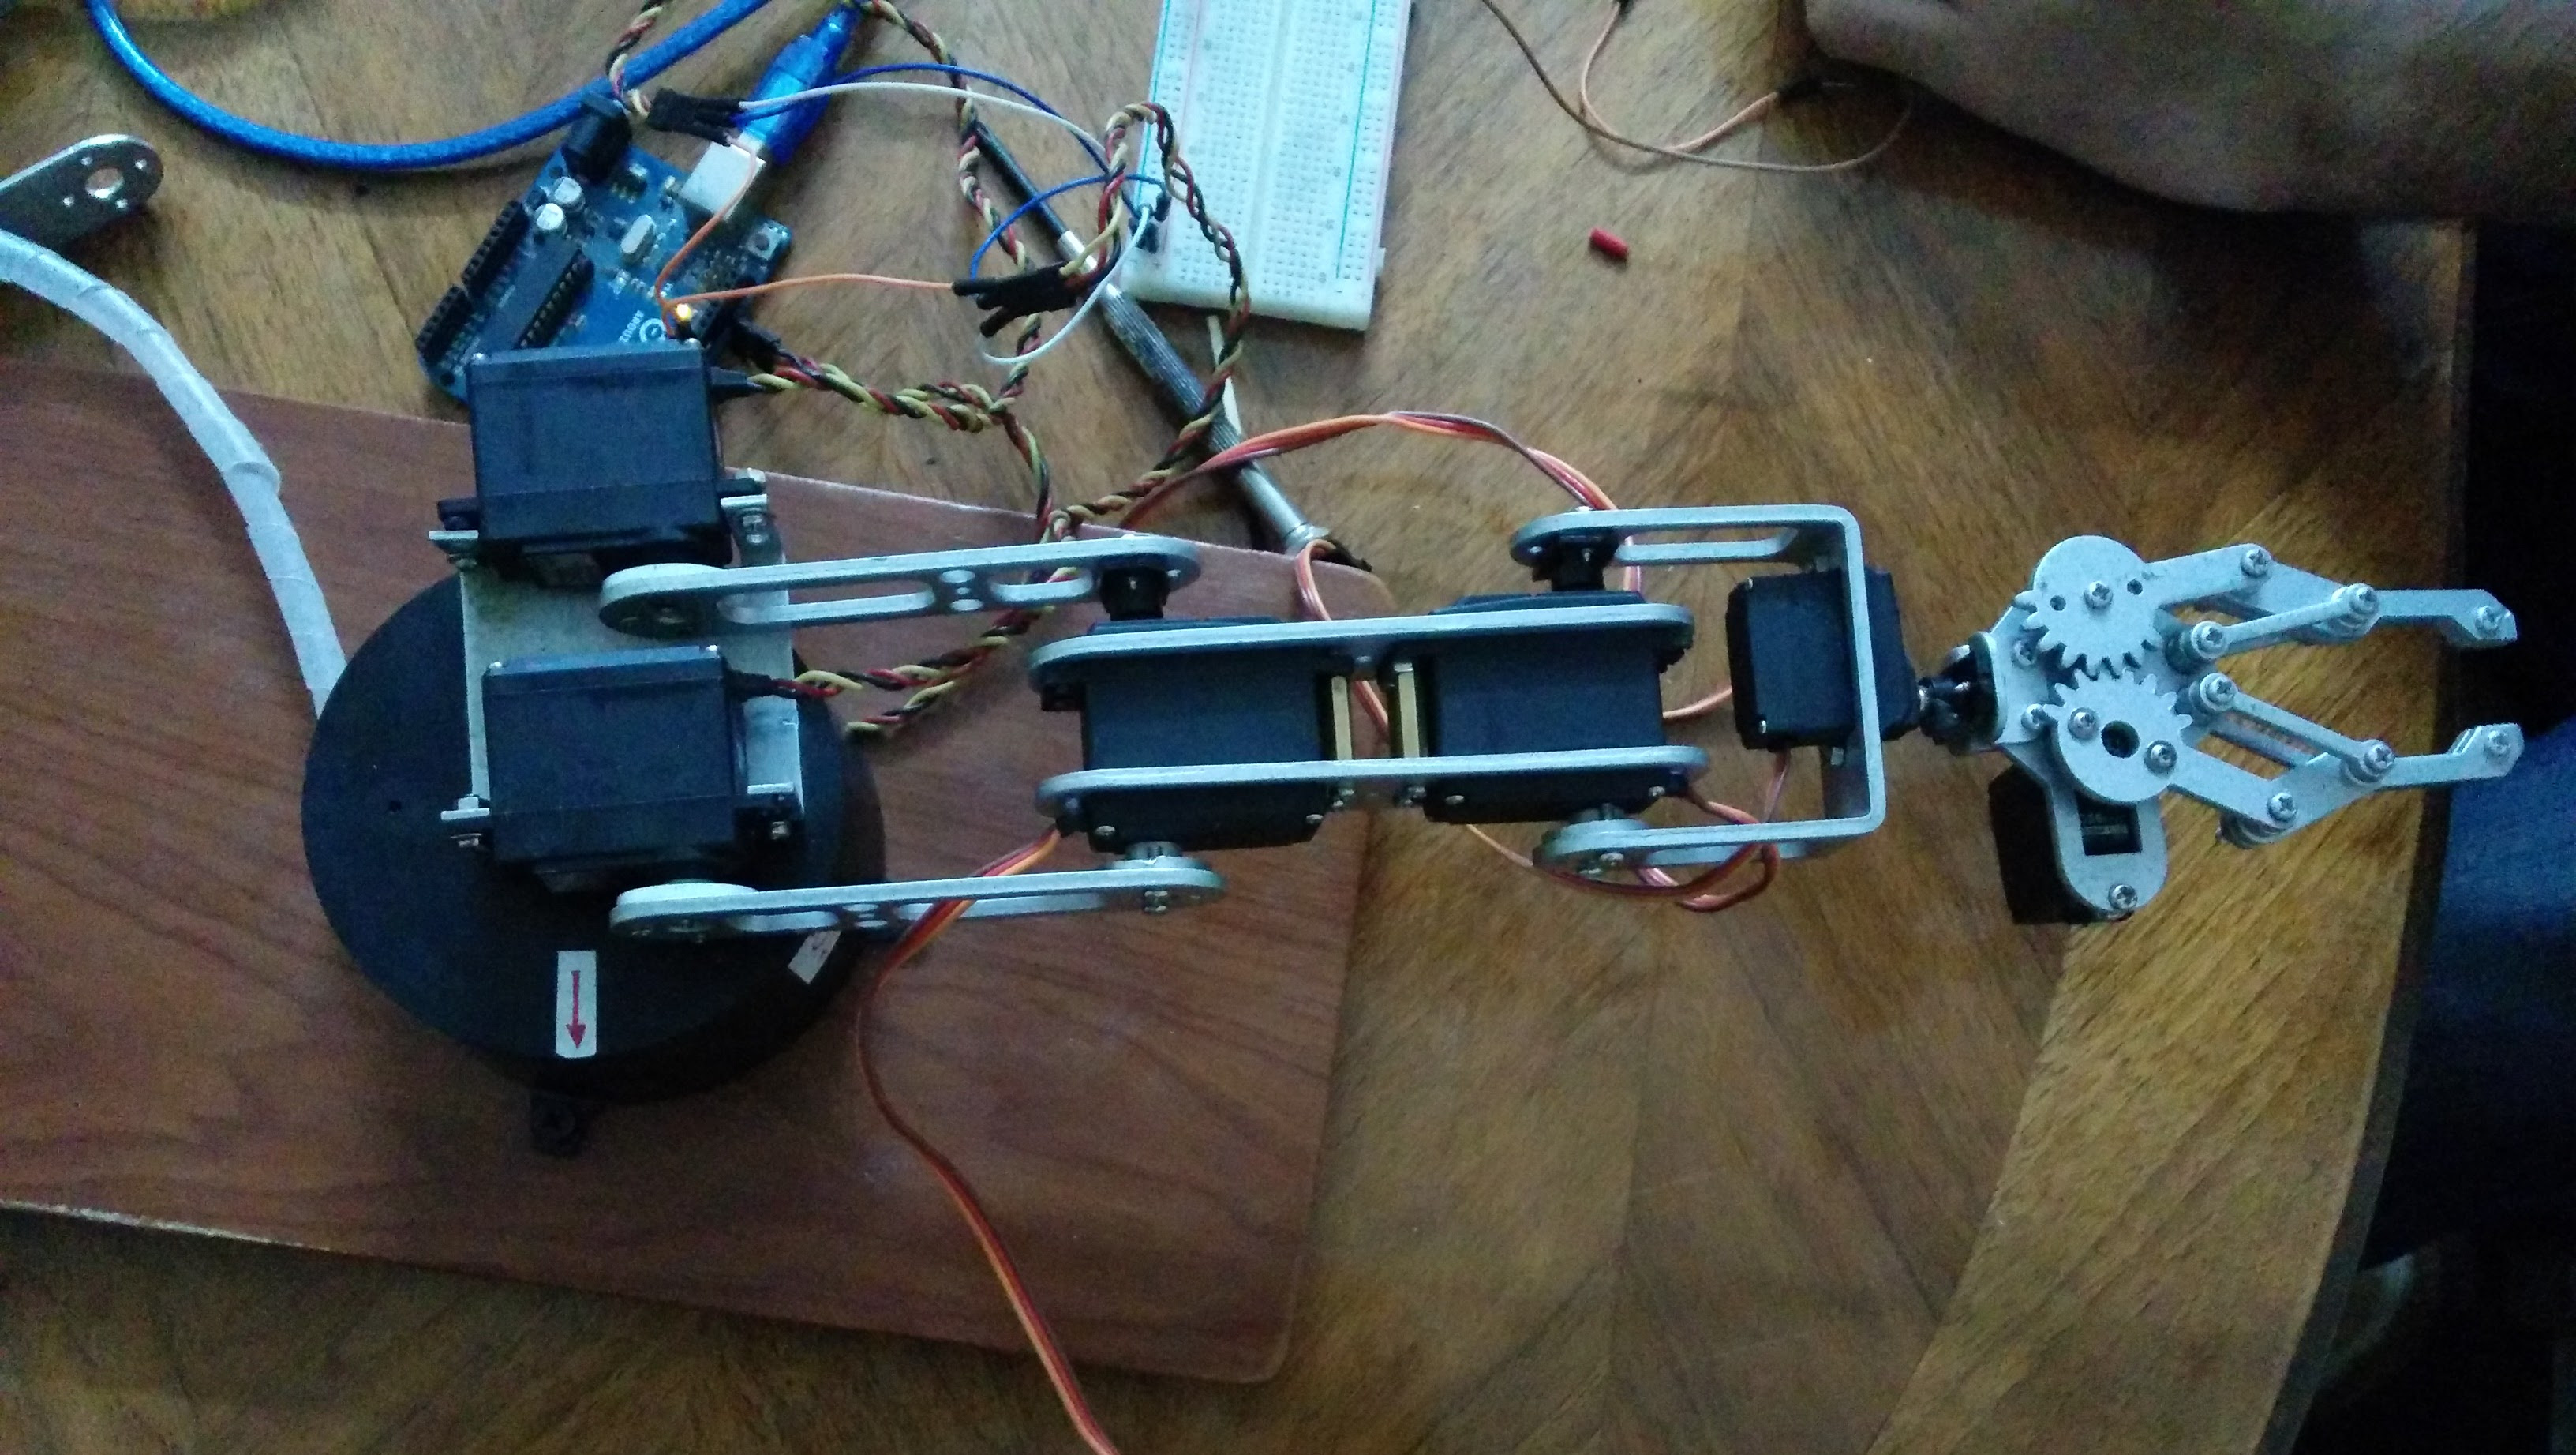
\includegraphics[width=0.8\textwidth]{Figures/Arm.jpg}}
\caption{The Arm}
\label{fig:arm}
\end{figure}
This low cost 5 Degrees of Freedom Robotic Arm is made from 3mm thick aluminum sheet, 6 servos are used for implementation: 4x DGServo S06NF STD servos for the base and the arm and the 2x DGServo S05NF STD micro servos operate the wrist and gripper. The robot arm is rougly 390 mm in length \cite{datasheet}\\
The arm's condition wasn't optimal, it was severely damaged due to negligence and misuse, some motors were completely damaged while others had severed wires. Repair methods are discussed in the following part.
\section{Arm repair}
\subsection{Arm State}
In this section we'll discuss the state at which the arm was given to us before we started fixing it.
\subsubsection{Actuators}
Testing started from bottom up by checking the data sheet of each motor and powering it up to observe its response:
\begin{itemize}
\item Motor 0: Shaft wasn't moving and the shaft screw hole was stuffed with super glue, the motor was dead
\item Motor 1 \& 2: Working but not in sync and the shaft was broken in motor 2
\item Motor 3: Dead, shaft screw hole was stuffed with super glue
\item Motor 4: Dead
\item Motor 5: Shaft not moving, makes noise and becomes very hot when we apply voltage to it.
\item Motor 6: Working, becomes hot when left working for a long time  
\end{itemize}
\subsubsection{Joints}
\begin{itemize}
\item Joint 0: Good but no screw to connect the shaft to the joint
\item Joint 1 \& 2: Good but the screws connecting the motor shaft to the joint were stripped 
\item Joint 3 \& 4: Good but no screws
\item Joint 5: Broken
\item Joint 6: In a good condition
\end{itemize}
\subsubsection{Links}
3 Links, where link 1 is composed of two links screwed together which resulted in an utterly long link. All the links were in a good condition.
\subsection{Repairing Phase 1}
\subsubsection{Actuators}
Motor 0:\\ 
After opening the motor we found that the motor gears were not intact and needed lubrication, the shaft was glued to the cover of the motor
\begin{itemize}
\item Removed the glue connecting the shaft to the cover using WD-40 spray and removed the glue stuffed in the shaft screw hole using a drill
\item Fixed the motor gears and lubricated them using silicon grease
\end{itemize}
Conclusion: Motor 0 is now working\\\\
Motors 3 \& 4: \\
After checking the gears and lubricating them the motors still didn't work, we tested the motors and the potentiometer and they were working fine We started testing the circuit boards of both motors\\
Motor 3: the common ground connecting the PCB to the motor body was disconnected so we soldered it back but still it didn't work. After several tests we found out that when holding the common ground with bare hand or connecting it to the earth ground the motor would rotate but still it didn't rotate correctly when given an angle so we concluded that there was a problem with the circuit board.\\
Motor 4: On testing the input and output of the PCB we observed that there was no voltage on the output pins so we concluded that that there was a problem with the PCB.\\
We excluded these motors from the arm and decided to use them as spare parts in case any motor had malfunctioned parts.\\\\
Motor 1 \& 2:\\
We exchanged the shaft of motor 2 with that of motor 4 then we synchronized the two motors by removing the links connected to them and giving them zero angles so that both of them would be fixed at their initial position and screwed the links back to them at this state.\\\\
Motor 5:\\
The motor shaft was glued to the link so it couldn't rotate and drew too much current which made it get very hot\\
We removed the glue, lubricated the gears with silicon grease and it worked like a charm\\\\
Motor 6:\\
After testing this motor which was the gripper's we found that the heat problem was due to the gripper gears being stiff and not well intact which was a design issue in the arm's gripper so we couldn't fix it so we advise that not let the gripper motor work for long periods\\\\

\subsubsection{Joints}
Joint 0 \& 3 \& 4: We purchased screws which fitted them\\
Joint 1 \& 2: We couldn't find screws which fitted these joints \\ 
Joint 5: We glued it using epoxy glue
\subsection{Repairing Phase 2}
After determining the actuators that are working we started checking the motors constraints and adjusting the initial position of each link, testing whether the motors torques were enough to lift the corresponding links:\\
\subsubsection{Constraints}
Motor 0: 180 degree\\
Motor 1 \& 2: 180 degrees\\
Motor 5: 180\\
Motor 6: 90 but for convenience use angle values ranging from 15 to 60 degrees\\
\subsubsection{Torque}
Motor 1, 2 torques weren't enough to lift the arm so we had to shorten link number 1 which composed of two links screwed together by removing the longer one which was a custom-made addition to the original design which we found at future electronics store \cite{datasheet}
\subsection{Repairing Phase 3}
We purchased two new motors to replace motor 3 \& 4 we also purchased new joints and replaced joint number 5 and screws which fitted joint 1 \& 2
\subsubsection{Constraints}
Motor 3: 120 degree\\
Motor 4: 180 degree\\
Note that: Motor 3 torque isn't high enough to lift the rest of the arm so we have to bend the rest of the arm to be able to lift it 
\section{Forward Kinematics}
The following figure is used to explain both forward and reverse kinematics\\
\begin{figure}[h]
\centering
{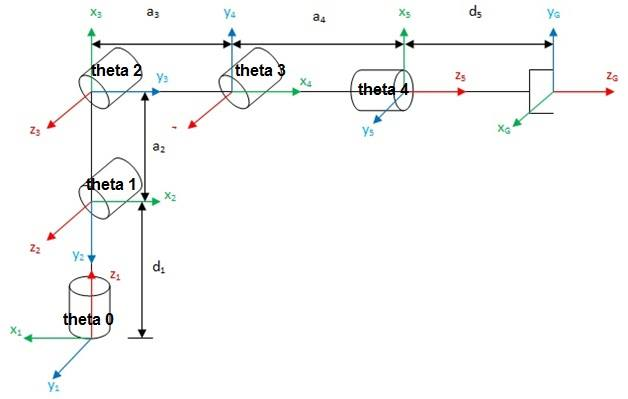
\includegraphics[width=0.8\textwidth]{Figures/Kine.jpg}}
\caption{Schematic \cite{picture}}
\label{fig:kine}
\end{figure}
The forward kinematics of the arm are as follows:\\\\
$\theta = \theta_1$ (\emph{yaw}) \\
$\phi = \theta_5$ (\emph{roll}) \\
$\psi = \theta_2 + \theta_3 + \theta_4 $ (\emph{pitch}) \\
Where: \\
$r = L_1C_2+L_2C_{2+3}+L_3C_{2+3+4}$ \\
$s = L_1S_2+L_2S_{2+3}+L_3S_{2+3+4}$ \\
$\therefore x=rc_1$ \\
\& $y=rs_2$ \\
\& $z=s$\\
\section{Inverse Kinematics}
\subsection{Existence of solution}
For a solution to exist x,y,z must be a part of the workspace: \{x,y,z\} $\in$ Workspace\\ 
The workspace is a half spherical shell with inner radius = $L_1-L_2-L_3$ and outer radius = $L_1+L_2+L_3$
\subsection{Singularity}
At $x=y=0$ we find that $\theta_1$ is undefined, we assume that $\theta_1=0$ in order to maintain a fixed roll angle
\subsection{Redundancy}
Each position has more than one solution with difference in $\phi$  so each unique solution is defined by x,y,z,$\phi$
\subsection{Equations}
We define the following:\\
s = z\\
$r = \sqrt[]{x^2+y^2}$\\
$\theta_1 = arctan2(y,x)$\\
$\theta_3 = arccos(\frac{(r-L_3c_{\phi})^2 + (s-L_3s_{\phi})^2 - {L_{1}}^2 - {L_{2}}^2 }{2L_1L_2})$\\
$\theta_2 = arcsin(\frac{(s-L_3s_{\phi})(L_1+L_2c_3)-L_2s_3(r-L_3c_{\phi})}{(r-L_3c_{\phi})^2 + (s-L_3s_{\phi})^2})$\\
$\theta_4 = \phi - \theta_2 - \theta_3$\\
$\theta_5 = \psi$\\
\subsection{Constraints}
$\theta_{1,2} \in [0,180]$\\
$\theta_{3,4} \in [0,120]$\\
Define:\\
$L_{max} = L_1 + L_2 + L_3$\\
$L_{min} = L_1 + cos(\frac{-2}{3}*\pi)*L_2 - L_3$\\
%$L_{min} = c_1 + c_{-120}-L_3$\\
$-L_{max} < x < L_{max}$\\
$-\sqrt[]{{(L_{max}}^2 - x^2)} < y < \sqrt[]{{(L_{max}}^2 - x^2)}$\\
If $r < L_{min}$ then $\sqrt[]{{L_{min}}^2 - r^2} < z < \sqrt[]{{L_{max}}^2 - r^2}$\\
If $L_{min} < r < L_{max}$ then $-\sqrt[]{(L_2+L_3)^2 - (L_1 - r)^2} < z < \sqrt[]{{L_{max}}^2 - r^2}$
\section{Implementation}
The code is split into two environments, a base station and an interface. This way the interface can be used by different base stations in different languages instead of forcing a single language.\\
It is also better in terms that the Matlab (base station) capabilities in calculation are much higher than Arduino (floating point precision).\\
The Arduino code is built in a way that makes it easy to adjust the pinout and the number of motors by changing a few lines at the beginning of the code.\\
\subsection{Connections}
\begin{figure}[h]
\centering
{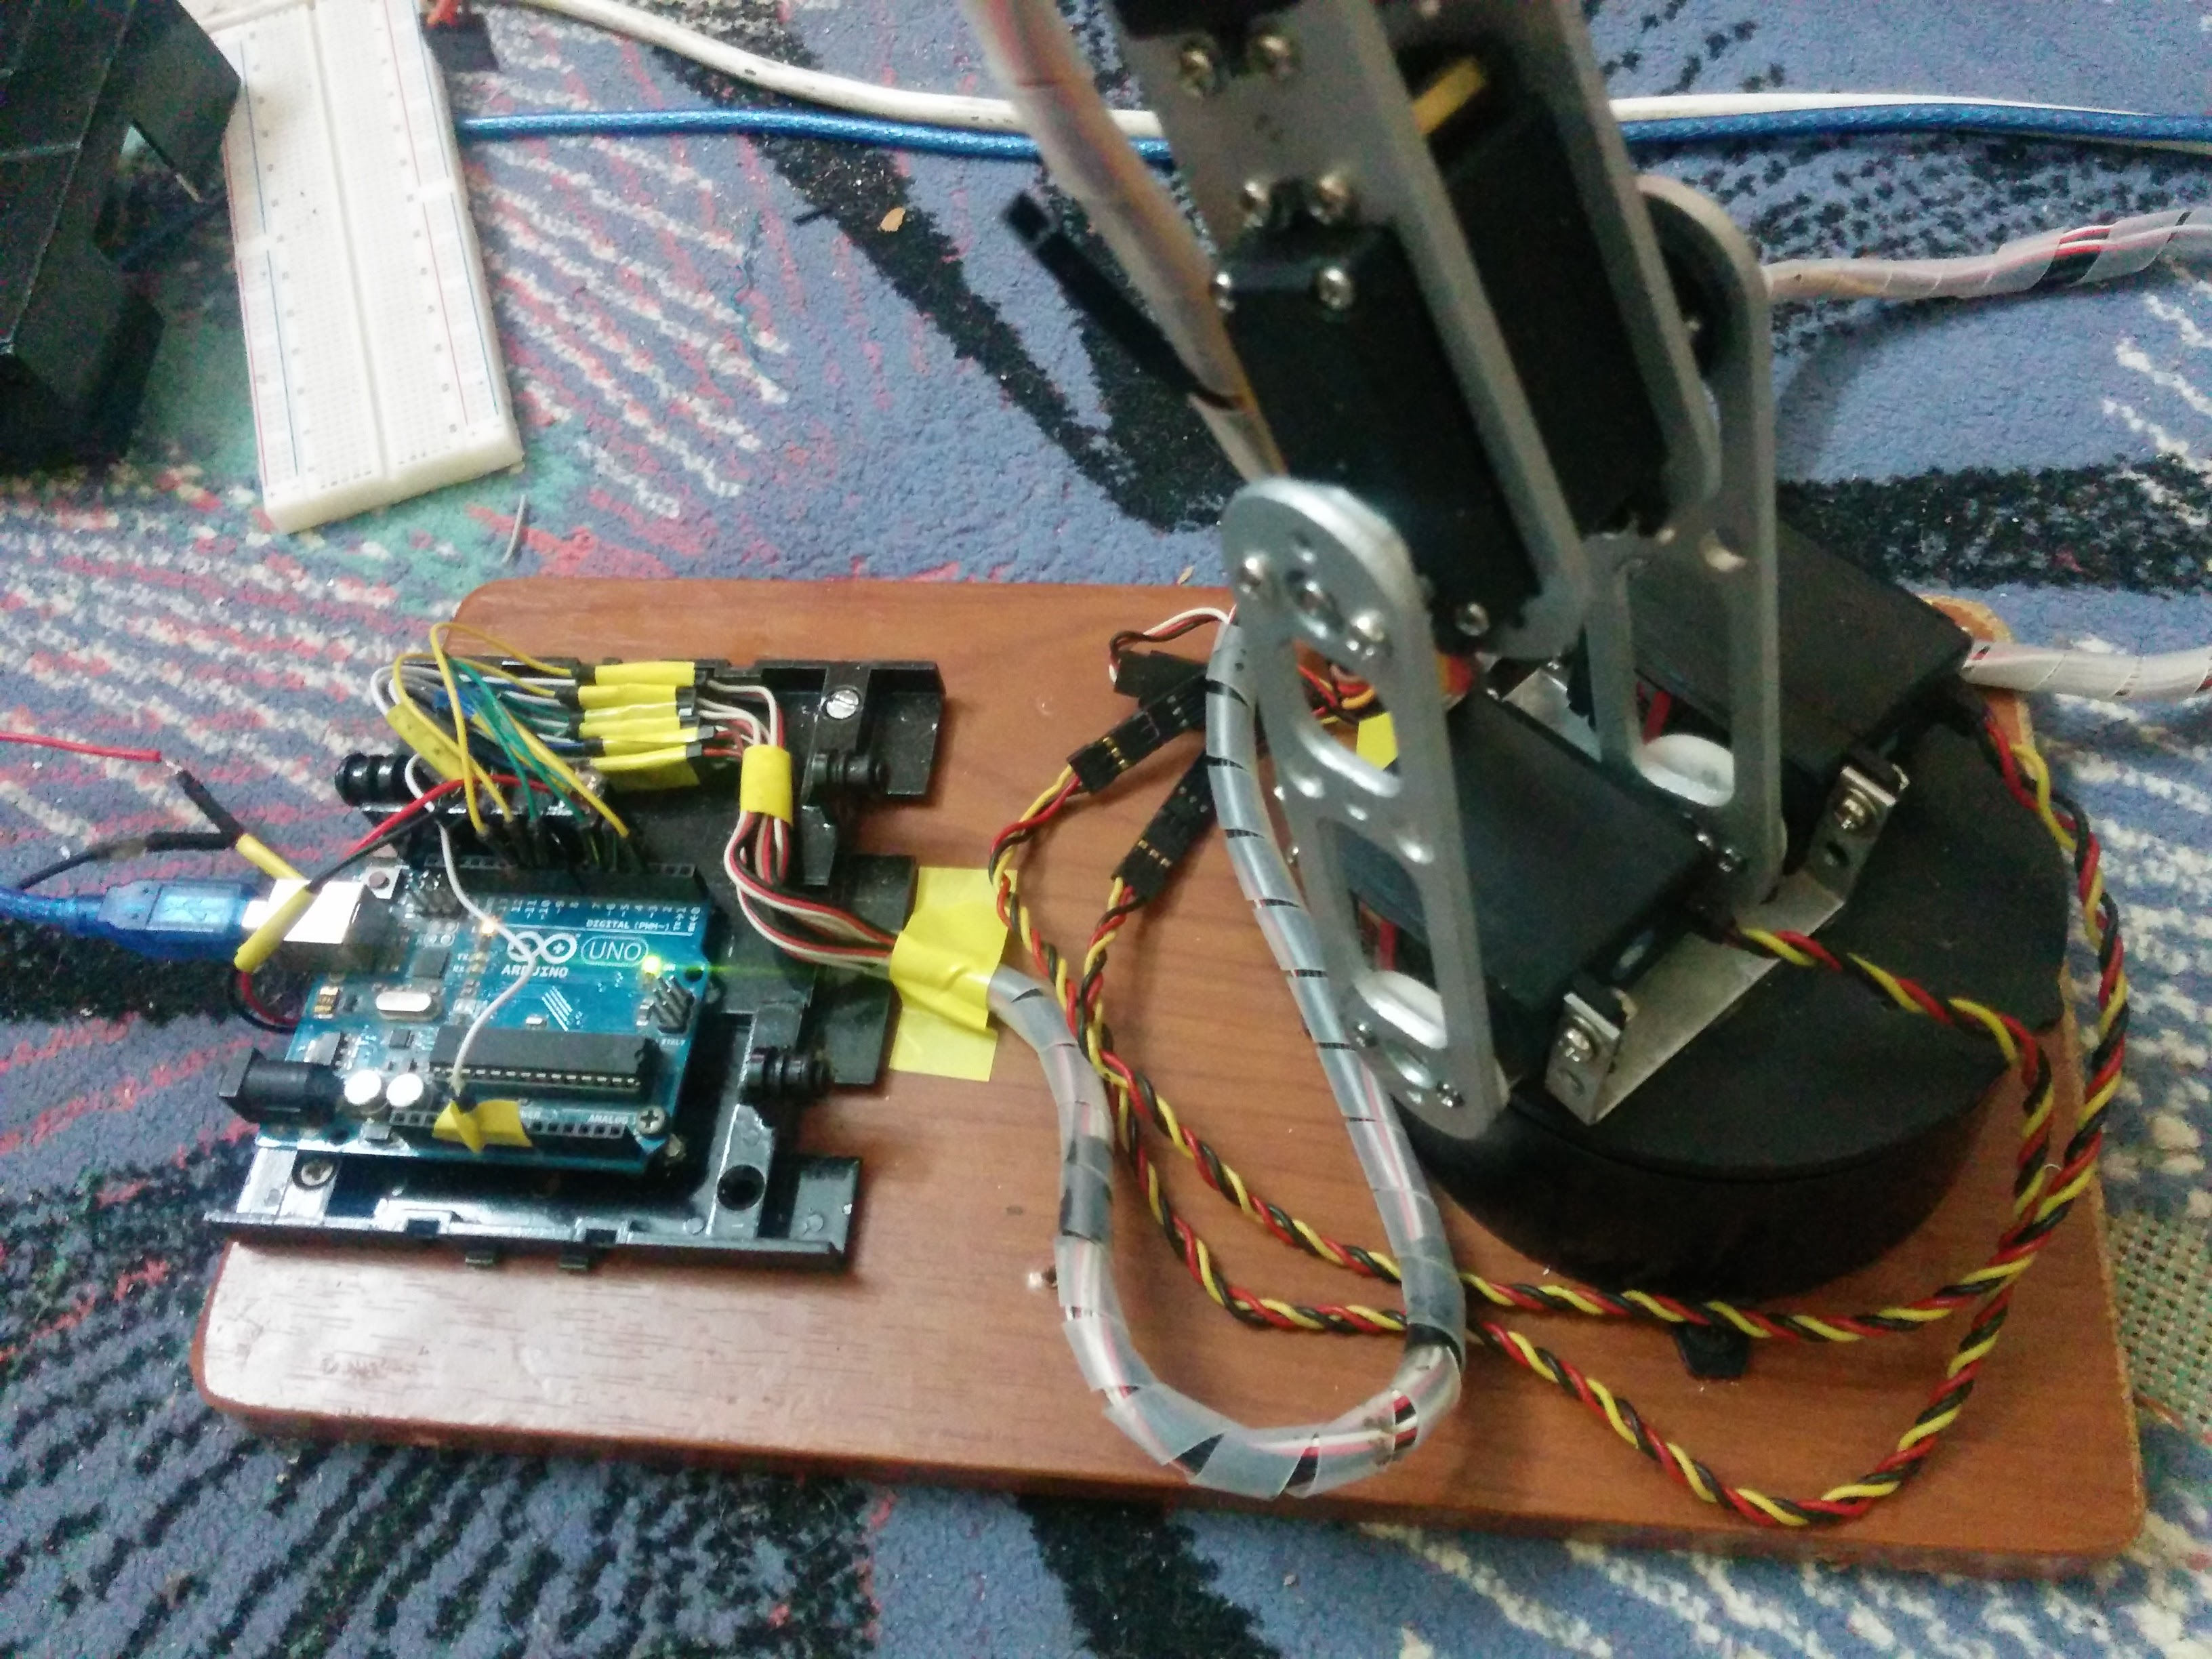
\includegraphics[width=0.8\textwidth]{Figures/Wire.jpg}}
\caption{Wiring}
\label{fig:wire}
\end{figure}
We built a box that encases all the wiring with only two outputs for serial and power. A servo motor consists of 3 Pins, a VCC, a ground and a signal pin .. so we connected all the VCC pins together to one output wire that connects to the power supply and all the ground pins together to one output wire that connects to the power supply's ground.\\
And the signal pins are connected to the Arduino randomly but are defined from the ground up at the beginning of the Arduino code. Motor datasheets can be found in the bibliography \cite{datasheet1} \cite{datasheet2}\\
The code exists on a Github repository \cite{github} to make it easier to collaborate our work and for others that are interested in continuing our work. 
\subsection{Arduino code}
The Arduino is built as an interface for the Base Station where its only purpose is to receive angles from the station and send them to the motors, the Arduino receives the angles through serial communication with a specific format of "xx yy:" where xx defines the motor number and yy defines the angle, with two separators, a space and a ":". As a concept the Arduino is used to control the actuator space, Figure \ref{fig:arduinoFlow} shows the flow chart of the code, the full code is available in Appendix \ref{appendix:arduino}\\
\begin{figure}[h]
\centering
{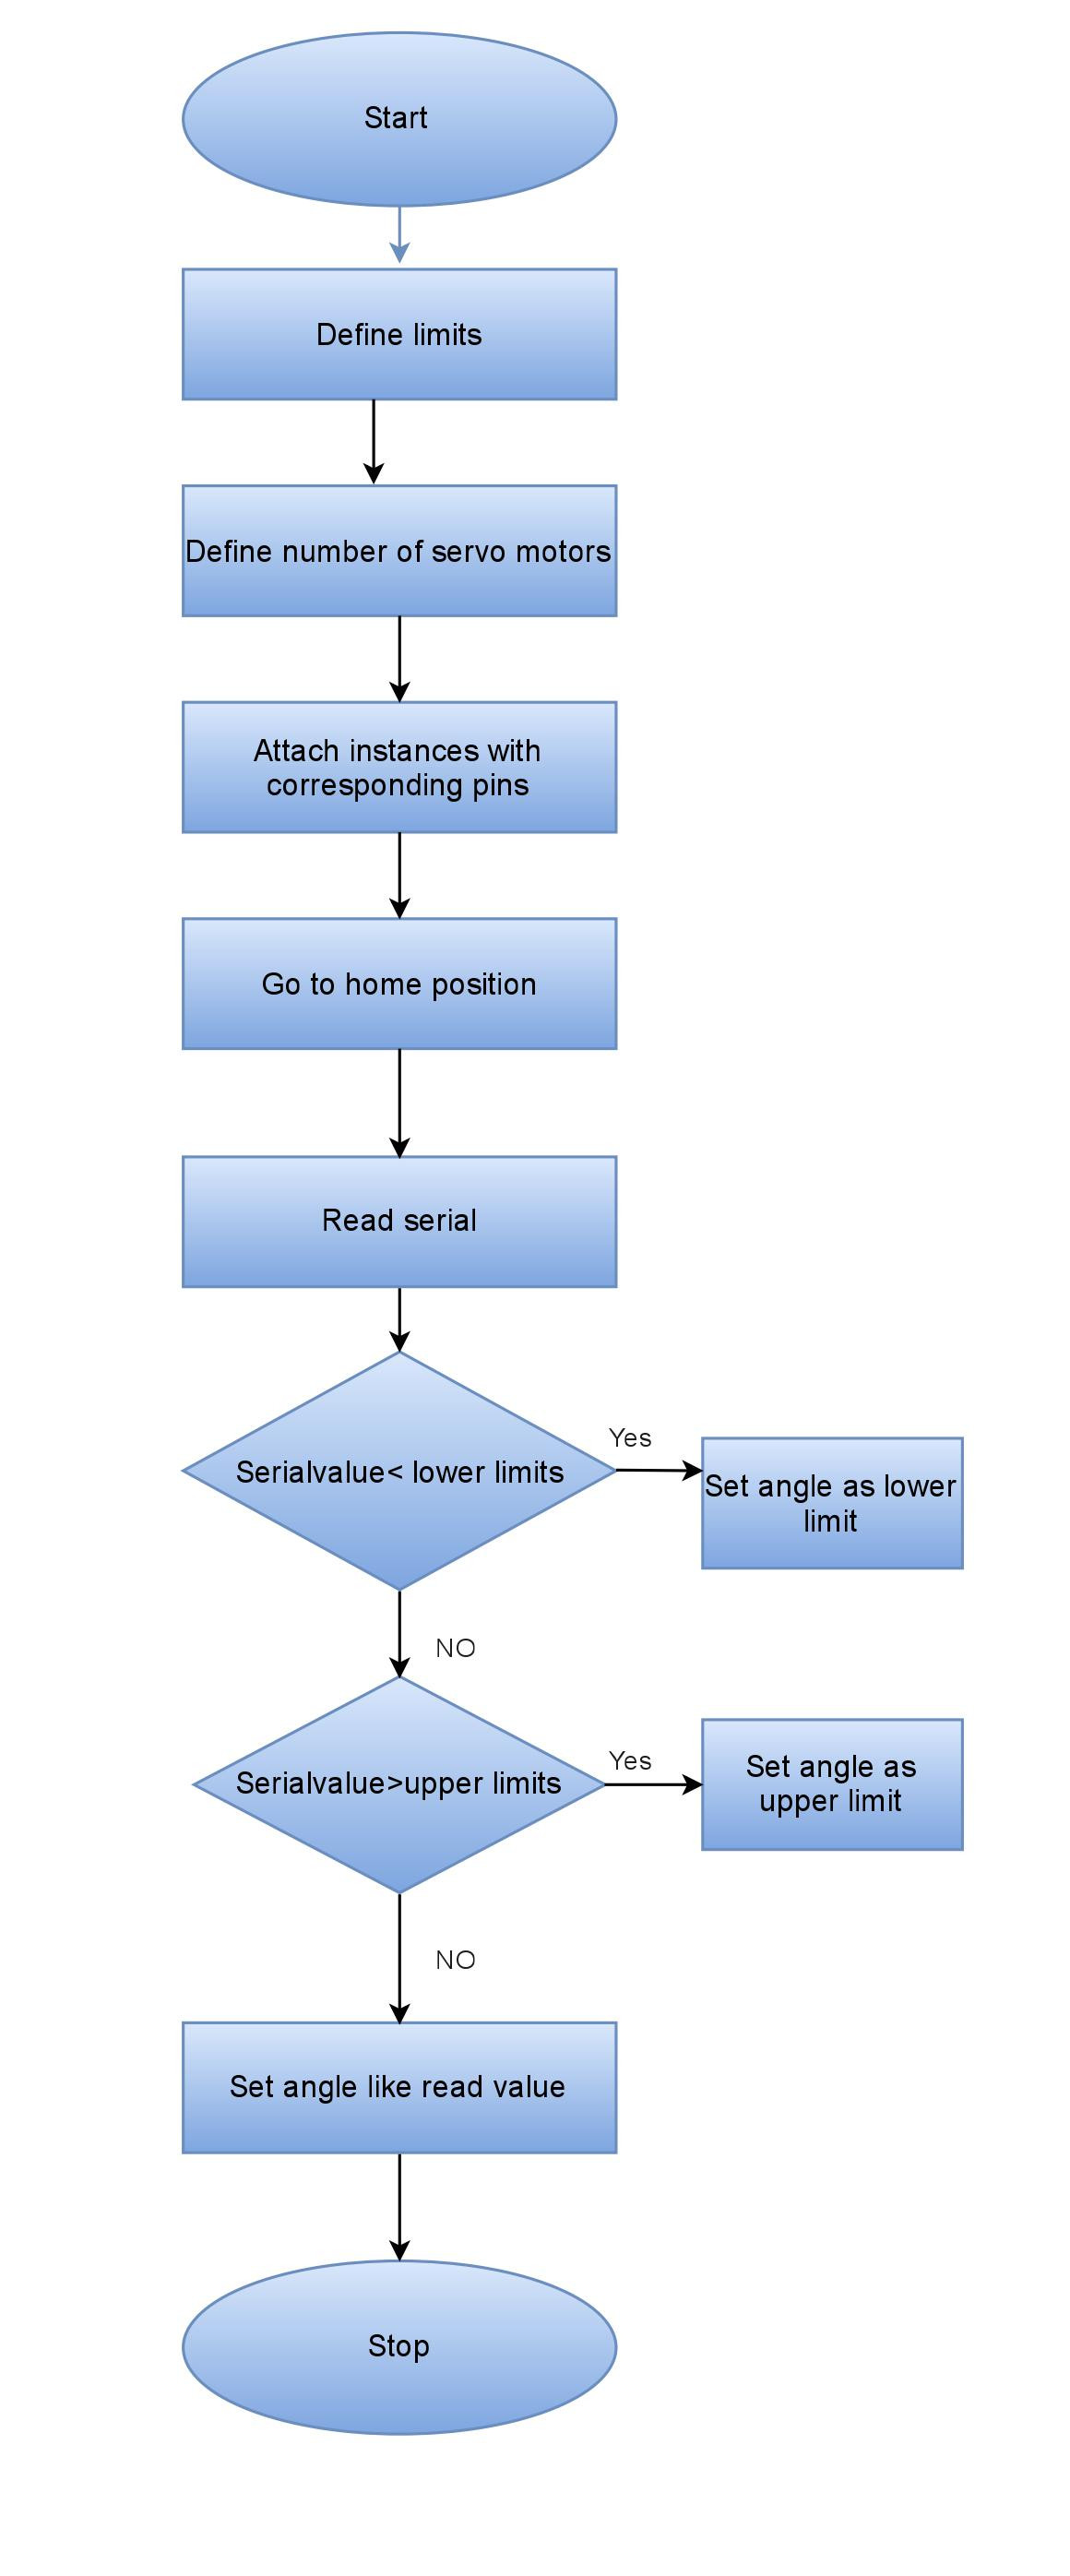
\includegraphics[width=0.4\textwidth]{Figures/Flow1.jpg}}
\caption{Arduino code Flow Chart}
\label{fig:arduinoFlow}
\end{figure}
A bug was found that whenever serial serial communication starts either through Arduino's interface or Matlab, the Arduino resets. this turned out to be a hardware problem that can be fixed by adding a 120 ohm resistance between 5V and reset headers. \cite{arduinoreset} 
\subsection{Matlab code}
We are using Matlab to convert x,y,z to appropriate angles for the motors and to interface with the user, the full code is available at Appendix \ref{appendix:matlab}.\\
The code simply uses the reverse kinematics equations we previously wrote and the constraints to find the appropriate angles for the Arduino and then sends them using Serial communication to the Arduino, it is built as a function so that in future development the function can be directly used by any higher level code like a GUI.
\section{Conclusion}
We were able repair the arm and get it up and running, but because of the lack of simulation we can't compare the results from both the simulation and the real arm to be able to determine whether or not it is working like it should.\\
We also found that the arm had loose joints and the gears in the motors sometimes break, probably due to bad motor quality or gears.
\subsection{Future improvements}
We suggest some improvements on the arm like:
\begin{itemize}
\item Build a better user interface (GUI) with more options like actions instead of single movements
\item Control the speed of the servo motor movements in a way that prevents the arm from falling fast when it's supposed to move down
\item Use the Matlab robotics toolbox to check the reverse kinematics and simulate the arm \cite{toolbox}
\item Fix the serial reset problem \cite{arduinoreset}
\item Use better power wires that have lesser resistance
\item Fix servo jitter problem that sometimes surfaces
\end{itemize}
\pagebreak
\appendix
\addtocontents{toc}{\protect\contentsline{chapter}{Appendix:}{}}
\section{Appendix}
\subsection{Arduino Code}
\label{appendix:arduino}
\begin{lstlisting}
//Servo.h is the library required to directly deal with servo motors
#include <Servo.h>
/*
 Pinout from base to grip:
 Motor 0 => 3
 Motor 1 & 2 => 5
 Motor 3 => 6
 Motor 4 => 9
 Motor 5 => 10
 Motor 6 => 11
 */
int thetaPin[] = {3,5,6,9,10,11};
// Introduce lower and upper limits for each motor due to mechanical
// limits
int lowerLimit[] = {0,0,0,0,0,16};
int upperLimit[] = {180,180,120,120,60};
// Number of motor pins
const int numberOfMotors = 6;
//We define a servo instance for each motor
Servo thetaServo[numberOfMotors];

void setup() {
  //Initialize Serial Com
  Serial.begin(9600);
  //Attach each instance with the corresponding pin
  for (int i = 0; i < numberOfMotors; i++) {
    thetaServo[i].attach(thetaPin[i]);
  }
  //Go to Home position
   for (int i = 0; i < numberOfMotors; i++) {
    thetaServo[i].write(lowerLimit[i]);
  } 
}
int Angle;
void loop() {
  /*
   Serial sends values in this format:
   xx yy:
   Where xx is the motor number, yy is the angle to be sent
   if xx is larger than the number of motors Arduino responds with
   Servo values
   */
  while (Serial.available()) {
   int servoNo = Serial.readStringUntil(' ').toInt();
   if (servoNo < numberOfMotors) {
     Angle = Serial.readStringUntil(':').toInt();
     // We check if the value of the Angle fits the limits
     if (Angle < lowerLimit[servoNo]) {
      thetaServo[servoNo].write(lowerLimit[servoNo]);
     } else if (Angle > upperLimit[servoNo]) {
      thetaServo[servoNo].write(upperLimit[servoNo]);
     } else {
      thetaServo[servoNo].write(Angle);
     }
     //For debugging purposes
//     Serial.print("Theta ");
//   Serial.print(servoNo);
//   Serial.print(" Was sent an angle of ");
//   Serial.println(Angle);
   } else {
    for (int i = 0; i < numberOfMotors; i++) {
      int val = thetaServo[i].read();
      Serial.println(val);
    }
   }
  }
}
\end{lstlisting}
\subsection{Matlab Code}
\label{appendix:matlab}
\lstset{frame=none,
  language=matlab,
  aboveskip=3mm,
  belowskip=3mm,
  showstringspaces=false,
  columns=flexible,
  basicstyle={\small\ttfamily},
  numbers=none,
  numberstyle=\tiny\color{gray},
  keywordstyle=\color{blue},
  commentstyle=\color{dkgreen},
  stringstyle=\color{mauve},
  breaklines=true,
  breakatwhitespace=true,
  tabsize=3
}
\begin{lstlisting}
function [] = goTo( x, y, z, pitch, phi, gripper )
%GOTO takes position and drive the ZUArm to go to it
%   Detailed explanation goes here

clc; 
close all

%% setup link lengths

L1 = 8; %the link length
L2 = 8.1; 
L3 = 17.2; 

Lmax = L1 + L2 + L3;

Lmin = L1 + cos(-(2/3)*pi) * L2 - L3;

%% Make sure that the position parameters within the Ropot workspace
% x must be in range [-Lmax, Lmax]

if(abs(x) > Lmax)
    fprintf('x is out of range');
    return
end

%% calculate y limits given x, read y value and make sure it's within limits

yLimit = sqrt(Lmax^2-x^2); %L^2 = x^2 + y^2 + z^2, z minimum value = 0 ==> y^2 = L^2-x^2
if (abs(y) > yLimit)
    fprintf('y is out of range');
    return
end

%% calculate z limits given x,

r = sqrt(x^2 + y^2);
zmaxLimit = sqrt(Lmax^2 - r^2);
if (r < Lmin)
    zminLimit = sqrt(Lmin^2 - r^2);
else
    zminLimit = -sqrt((L2+L3)^2 - (L1-r)^2);
end
    
% solve approximation errors
if ~isreal(zminLimit)
    zminLimit = 0;
end
if ~isreal(zmaxLimit)
    zmaxLimit = 0;
end
    
if ((z < zminLimit) || (z > zmaxLimit))
    fprintf('z is out of range');
    return
end

%% check that roll angle within the joint angle limits

if ~isempty(phi)
    if (phi > 180 || phi < 0)
        fprintf('roll angle is out of range');
        return
    end
end

%% check gripper angle

if ~isempty(gripper)
    if ( gripper < 0 || gripper > 180)
        fprintf('gripper angle out of range\n');
    end
end

%% read pitch angle

if ~isempty(pitch)
    if (pitch < -180 || pitch > 180) %accept all values for testing
        fprintf('pitch angle out of range\n');
        return
    end
end
pitch = pitch * (pi/180); %degres to radian
    
%check pitch limits -not reliable and need modification-
pitchmax1 = acos((r+L1+L2) / L3);
pitchmin1 = acos((r - L1 - L2) / L3);

pitchmax2 = asin((z+L2)/L3);
pitchmin2 = asin((z-L1-L2)/L3);

pitchmax = min(pitchmax1, pitchmax2);
pitchmin = max(pitchmin1, pitchmin2);

%% Inverse kinematics 
errorFlag = 0;

outstr= [];

if y < 0
    theta0 = atan2(-y,-x);
else
    theta0 = atan2(y,x);
end
    
theta2 = acos(((r-L3*cos(pitch))^2+(z-L3*sin(pitch))^2-L1^2-L2^2)/(2*L1*L2));
theta1 = asin(((z-L3*sin(pitch))*(L1+L2*cos(theta2))-L2*sin(theta2)*(r-L3*cos(pitch)))/((r-L3*cos(pitch))^2+(z-L3*sin(pitch))^2));
if y < 0
    theta1 = pi - theta1;
end
    
% check for errors due to pitch out of range
if ~isreal(theta2) || ~isreal(theta1) || ~isreal(theta0)
    errorFlag = 1;
    fprintf('pitch angle out of range, chose another angle');
end
    
theta3 = pitch - theta2 - theta1;
                    
% check constraints
    
if (~errorFlag) %&& ((pitchmin < pitch) && (pitch < pitchmax))
    %check for joints angles constraints
    if (pi < theta0 || 0 > theta0)
        errorFlag = 1;
    end

    if (pi < theta1 || 0 > theta1)
        errorFlag = 1;
    end

    if (0 < theta2 || (-(2/3)*pi) > theta2)
        errorFlag = 1;
    end

    if (0 < theta3 || (-pi) > theta3)
        errorFlag = 1;
    end

    if ~errorFlag 
        %forward kinematics for douple check
        pitchC = theta1+theta2+theta3;
        rC = L1*cos(theta1) + L2*cos(theta1+theta2) + L3*cos(pitchC);
        zC = L1*sin(theta1) + L2*sin(theta1+theta2) + L3*sin(pitchC);
        xC = rC*cos(theta0);
        yC = rC*sin(theta0);
    
        if theta1 > pi/2
            xC = -xC;
            yC = -yC;
        end
    
        %consider small error due to approximation
        if(abs(pitchC-pitch)>0.1 || abs(zC-z)>0.1 || abs(xC-x)>0.1 || abs(yC-y)>0.1 || ~isreal(zC) || ~isreal(xC) || ~isreal(yC))
            fprintf('problem \n')
            errorFlag = 1;
        end
    end
end
%radian to degres to be suitable for servo motor
theta0 = round(theta0 * (180/pi));
theta1 = round(theta1 * (180/pi));
theta2 = round(theta2 * (180/pi));
theta3 = round(theta3 * (180/pi));

if theta0 < 0
    theta0 = -theta0;
end

if theta1 < 0
    theta1 = -theta1;
end

if theta2 < 0
    theta2 = -theta2;
end

if theta3 < 0
    theta3 = -theta3;
end

%output string that should be sent to arduino
outstr = [outstr, '0 ', num2str(theta0), ':1 ',int2str(theta1) ,':2 ',int2str(theta2) ,':3 ' ,int2str(theta3) ,':'];


if errorFlag
    errorFlag
end

if ~isempty(phi)
    theta4 = round(phi);
    outstr = [outstr, '4 ', num2str(theta4), ':'];
end

if ~isempty(gripper)
    outstr = [outstr, '5 ', num2str(gripper), ':'];
end

%% Connecting to Arduino via serial communication
% output string sent to Arduino is at form "0 theta0:1 theta1:2 theta2:3
% theta3:4 theta4:5 gripper" not all terms must appear
outstr
delete(instrfind)
global S
if (~errorFlag || 1)
    S = serial('COM28','BaudRate',9600,'timeOut',0.05);
    fopen(S);
    pause(2);
    fprintf(S, outstr);
    pause(1);
    fclose(S);
end
end
\end{lstlisting}
\begin{thebibliography}{9}
\bibitem{github}
ZUArm github repository
\url {https://github.com/OsamaYousry/ZUArm}
\bibitem{datasheet}
Future Electronics - 6DOF Arm \url{http://store.fut-electronics.com/collections/robot-arm/products/6dof-robot-arm-with-gripper-and-controller}
\bibitem{}
6 DOF Arm documentation
\url{http://glicture.com/4494407.html}
\bibitem{datasheet1}
HS645MG Motor datasheet
\url{http://www.robotshop.com/media/files/pdf/hs645mg.pdf}
\bibitem{datasheet2}
S06NFSTD Motor datasheet
\url{https://dlnmh9ip6v2uc.cloudfront.net/datasheets/Robotics/S06NFSTD.pdf}
\bibitem{picture}
Kinematics photo \url{https://www.researchgate.net/post/Can_anyone_help_me_find_the_inverse_kinematic_solution_of_a_5_DOF_robot_arm}
\bibitem{arduinoreset}
Disable Arduino Reset 
\url{http://playground.arduino.cc/Main/DisablingAutoResetOnSerialConnection}
\bibitem{toolbox}
Matlab robotics toolbox documentation
\url{http://www.petercorke.com/RTB/r9/html/SerialLink.html}
\bibitem{}
Matlab serial documentation
\url{www.mathworks.com/help/matlab/serial-port-devices.html}
\bibitem{}
Arduino servo library
\url{https://www.arduino.cc/en/Reference/Servo}
\end{thebibliography}
\end{document}